\chapter{Introduction}

%% ============================================================
\section{Background and Motivation}\label{sec:intro_motivation}
%% ============================================================

This thesis is organized around a single progression. Automating industrial component handling first demands reliable \emph{perception} with a single arm, followed by the introduction of a second arm to cover the workspace that one arm cannot. This addition raises a \emph{coordination} concern no single-arm system ever faces, instantly making \emph{safety} a live issue the moment two arms share a workspace. Consequently, this calls for \emph{motion planning} capable of using a safety signal to keep the arms apart while they move. Ultimately, this progression exposes exactly where a hand-designed, classical control law runs out of headroom and a \emph{learned} one is warranted.

Each stage is a precondition for the next rather than an independent application: a component cannot be manipulated before it is localized; a second arm cannot be added safely before it is decided which arm acts; and concurrent motion cannot be trusted without a continuous distance signal. Furthermore, that safety signal is only useful once a planner consumes it. Only with a working classical planner in hand does it become possible to identify, precisely, the coordination problem that classical control cannot solve on its own. This thesis traces that progression from start to finish, from a single arm sorting bolts by classical computer vision to a pair of arms coordinating a pre-assembly alignment through reinforcement learning.


This thesis begins at the exact point where conventional robotic deployments begin to strain. While industrial robots reduce human fatigue and are forecast to grow into a USD 55.4 billion industry by 2032~\citep{develop2024robotic}, conventional, hard-coded single-arm systems no longer satisfy the demands of unstructured, high-throughput manufacturing~\citep{abbas2023systematic}. A single arm's reach is strictly fixed; as work cells scale up, the spatial distribution of components and complexity of the task routinely exceeds what one manipulator can physically cover/handle. Modern manufacturing increasingly demands collaborative task execution such as cooperative assembly alignment, where an operation inherently requires the simultaneous coordination of two arms. The standard industrial response for deploying a second arm within the same workspace, transforms a baseline perception based pick and place problem into a coordination problem, coordination into a safety problem, and safety into a motion planning problem. Each of these challenges is addressed sequentially by the studies comprising this thesis~\citep{surya2025iapf,sk2025competitive}. Finally, only when classical perception, coordination, safety, and planning frameworks are established does the fundamental limitation emerge: a fixed, hand-designed control law cannot inherently generalize across continuous trajectories or co-evolve a coordination strategy with a control prior. Learned control directly resolves this limitation~\citep{sk2025diktracking,sk2026priorguided}.

This thesis develops that progression across four connected themes. It begins with
\emph{perception} for small, low-textured industrial components such as fasteners, moves from a single arm to a \emph{dual-arm} system and the coordination question this raises, establishes the \emph{safety and motion-planning} paradigm that shared-workspace operation demands, and finally replaces the classical control layer with \emph{learned} controllers for both single-arm trajectory tracking and cooperative dual-arm alignment. Figure~\ref{fig:intro_roadmap} shows how the eight constituent studies map onto this progression, and Table~\ref{tab:intro_studies} summarizes each of them.

\begin{figure}[htbp]
\centering
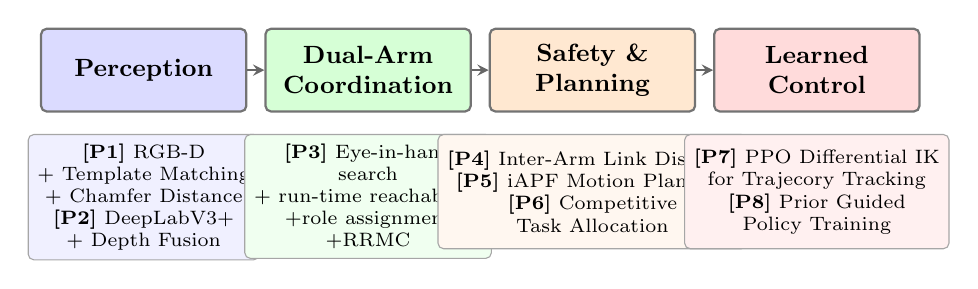
\begin{tikzpicture}[
  >=stealth,
  themebox/.style={rectangle, rounded corners=2pt, draw=black!55, thick,
                   minimum width=0.215\textwidth, minimum height=1.05cm,
                   align=center, font=\small\bfseries, anchor=north},
  studybox/.style={rectangle, rounded corners=2pt, draw=black!35,
                   minimum width=0.215\textwidth, minimum height=1.45cm,
                   align=center, font=\scriptsize, anchor=north},
  flow/.style={->, thick, draw=black!60}
]
\node[themebox, fill=blue!14]   (t1) at (0,0)                {Perception};
\node[themebox, fill=green!16]  (t2) at (0.235\textwidth,0)  {Dual-Arm\\Coordination};
\node[themebox, fill=orange!18] (t3) at (0.470\textwidth,0)  {Safety \&\\Planning};
\node[themebox, fill=red!14]    (t4) at (0.705\textwidth,0)  {Learned\\Control};

\node[studybox, fill=blue!6]   (s1) at (0,-1.35)               {\textbf{[P1]} RGB-D\\ {+} Template Matching\\ {+} Chamfer Distance\\\textbf{[P2]} DeepLabV3{+}\\{+} Depth Fusion};
\node[studybox, fill=green!6]  (s2) at (0.235\textwidth,-1.35) {\textbf{[P3]} Eye-in-hand\\search\\ {+} run-time reachability\\{+}role assignment \\{+}RRMC};
\node[studybox, fill=orange!6] (s3) at (0.470\textwidth,-1.35) {\textbf{[P4]} Inter-Arm Link Distance\\\textbf{[P5]} iAPF Motion Planning\\\textbf{[P6]} Competitive\\ Task Allocation};
\node[studybox, fill=red!6]    (s4) at (0.705\textwidth,-1.35) {\textbf{[P7]} PPO Differential IK\\ for Trajecory Tracking \\\textbf{[P8]} Prior Guided\\ Policy Training};

\draw[flow] (t1.east) -- (t2.west);
\draw[flow] (t2.east) -- (t3.west);
\draw[flow] (t3.east) -- (t4.west);
\end{tikzpicture}
\caption{Scope and progression of the work presented in this thesis. Each theme supplies a
component consumed by the next. Perception localizes the components, dual-arm coordination decides
which arm acts, the safety and planning layer keeps the arms apart while they move, and the learned
controllers replace the classical control layer beneath all of it.}
\label{fig:intro_roadmap}
\end{figure}

%% ============================================================
\section{Perception for Industrial Component Handling}\label{sec:intro_perception}
%% ============================================================

Efficient object manipulation is a crucial component of modern industrial automation. Precise
object detection, size estimation, and sorting are essential for a range of processes including
component assembly, packaging, and quality control. In particular, sorting small, low-textured
objects in densely packed environments, common in warehouses, assembly lines, and logistics
operations, remains a significant challenge. Manual sorting is labour-intensive, error-prone,
and can lead to production bottlenecks, while inaccurate sorting results in delayed production,
increased costs, and reduced overall efficiency.

Fasteners such as nuts and bolts are the canonical instance of this problem. They are critical
components in industrial assembly processes, yet their detection and segmentation in factory
environments is difficult precisely because they have limited visual features and frequently
overlap. Existing methods for object sorting suffer from limitations in accuracy, speed, and
adaptability to complex environments, and many require multiple sensors, increasing system
complexity and cost.

%% ------------------------------------------------------------
\subsection{The Limits of Classical Vision}\label{subsec:intro_classical}
%% ------------------------------------------------------------

Classical vision techniques, markers, edge detection, corner detection, and contour detection,
may not be reliable in all situations. Under varying light conditions, shapes, and colours
these methods can underperform at localization, producing faulty localization and size
estimation~\citep{omahony2020deep}. The difficulty is well documented across the object detection and pose estimation literature. \citet{sumi2002object} used stereo vision to determine the 6-DOF pose of an object placed in a cluttered scene even under occlusion, demonstrating good accuracy in pose estimation and improved recognition rates, but the work faces challenges related to computational complexity and is limited to certain lighting conditions. \citet{hu2018segmentation} introduced a segmentation-driven approach to 6D pose estimation which, by predicting 2D keypoint locations for visible object parts and combining them using confidence scores, achieved robust pose estimation and state-of-the-art performance on challenging datasets, although its reliance on accurate segmentation and its potential sensitivity to occlusions and initial conditions remain
limitations.

Surface texture is a crucial feature for object recognition, but many industrial components lack
distinctive textural patterns. \citet{wohlhart2015learning} proposed learning descriptors using a
CNN to address this challenge, demonstrating potential for recovering pose information but with high
computational complexity and a strong reliance on the dataset. The method's robustness was further
compromised by lighting variation, occlusions, and background clutter, all of which affect
descriptor accuracy. \citet{back2020segmenting} proposed a synthetic data generation pipeline and
an RGB-D Fusion Mask R-CNN to address the segmentation of texture-less industrial components. By
randomizing textures in synthetic data the focus shifted to shape-based features, and a confidence
map estimator enhanced the model's ability to exploit depth information for improved segmentation.
While promising, the reliance on synthetic data for training raises concerns about domain adaptation
to real-world scenarios.

Shape-based object segmentation can be advantageous in scenarios with poor figure-ground contrast
or illumination~\citep{borenstein2006shape}, although while such a framework performs well on the
shapes it has been trained on, its ability to generalize to completely unseen shapes may be limited.
\citet{wohlkinger2011shape} instead viewed the classification task as a matching problem,
introducing a method that identifies similar 3D models from comparable viewpoints by analysing
specific surface features. Although the method incorporates inter-view similarity, it may still
struggle with extreme variations in viewpoint, and objects viewed from angles significantly
different from those in the training set may not be matched accurately. The approach may also have
limitations in handling severe occlusions where significant parts of the object are not visible in
the depth image.

Most bin-picking applications have used the concept of matching a template of the expected object in
the scene to estimate its 3D pose, as this is simpler and does not require any previously trained
models~\citep{liu2012fast,guo2020fast,nguyen2022templates}. This methodology can be preferable in
industry because the CAD models used as templates are typically already available for the components
being handled~\citep{yan2020fastobjectpose}.

The first study of this thesis takes that route. It presents a novel approach for automated bolt
handling using 3D point-cloud data acquired from an RGB-D camera, employing $k$-means clustering
for segmentation and Oriented Chamfer matching for precise pose estimation, enabling a 6-DOF Kinova Gen3 Lite arm to accurately pick and place bolts, with colour-based segmentation and contour analysis facilitating size estimation for subsequent sorting. The method leverages the rich information provided by RGB-D cameras to improve object segmentation accuracy and reduce reliance on multiple sensors. Experiments conducted in a simulated shop-floor table top environment using Gazebo (ROS1) with a Kinova Gen3 Lite arm demonstrated the system's ability to handle overlapping bolts and achieved bolt sorting without any misclassifications~\citep{sk2024bolthandling}.

%% ------------------------------------------------------------
\subsection{Learned Segmentation Fused with Classical Vision}\label{subsec:intro_learned_vision}
%% ------------------------------------------------------------

It is instructive to contrast the machine's difficulty with how humans complete the same task. On
first identifying an object, a person relies on prior knowledge to recognize its shape and texture
and thereby conclude which category it belongs to. Size is then estimated either by visual
assessment or by physically handling the object. This process is skill-based and prone to mistakes.
Integrating human-like perception with classical vision techniques to estimate size in random
environments with fewer mistakes would represent a significant advancement in
automation.

Recent advances in deep learning, and Convolutional Neural Networks (CNNs) in particular, offer a
route past the limitations of purely classical methods. CNNs can learn to extract relevant features
from images even for small objects with limited detail, and combining this with sensor fusion
provides a more robust understanding of object size and shape. Integrating CNNs with classical
vision not only facilitates feature extraction for small, limited-feature objects but also supports
accurate size estimation, streamlining the subsequent actions taken on the basis of the detected
size.

Image segmentation is the fundamental technique here, partitioning an image into distinct regions
based on the class to which each pixel belongs. Segmentation can be achieved in two ways, instance
segmentation, which would classify all bolts within a cluttered image and assign a unique colour and
label to each individual bolt, and semantic segmentation, which assigns a single label and colour to
all bolts in the image~\citep{yin2022bridging}. Because the objective is to sort bolts according to
their size rather than to distinguish individual instances, a unique label per bolt is not required,
and using semantic segmentation simplifies the segmentation process and reduces computational
complexity. Encoder-decoder CNN architectures have performed best for
classical image segmentation, spanning FCN~\citep{long2015fully}, deconvolution
networks~\citep{noh2015learning}, U-Net~\citep{ronneberger2015unet}, and the DeepLab
family~\citep{mo2022review}. Alongside these, PPLiteSeg (STDC~I and~II)~\citep{peng2022ppliteseg}
provides lightweight CNN architectures designed for real-time applications in resource-constrained
environments, while OCRNet~\citep{yuan2020ocrnet} leverages an object-contextual representation
approach, demonstrating the potential benefits of exploring techniques beyond classical CNN-based
architectures.

Size estimation from 2D segmented images, leveraging classical vision techniques, is the second key
component. Comparisons of traditional classical vision methods with deep learning
methods~\citep{omahony2020deep} highlight the advantages of integrating both approaches, and
explain how the combination can enhance computer vision perception, leading to more robust and
accurate results. Deep-learning-based object detection can be used to estimate object size from
bounding box dimensions and aspect ratio with some success, as demonstrated using RGB-D cameras for
size estimation~\citep{wang2017tree}. Applying classical vision to a deep-learning-based
\emph{segmentation} instead provides more accurate object boundaries than direct bounding boxes,
which leads to accurate size estimation and eliminates the influence of background clutter on size
measurements.

The concrete challenges in this task are therefore fivefold, overcoming lighting conditions and
cluttered environments in the factory setup, extracting features from small and less-featured
objects, dealing with colour variations between old and new bolts, achieving precise size
estimation of small objects, and integrating the perception module with the
robot.

The second study addresses these directly, amalgamating deep-learning-based segmentation with
classical vision for automated bolt sorting in an unstructured industrial environment. PPLiteSeg
(STDC~I and~II), OCRNet, and DeepLabV3+ were evaluated on a custom bolt dataset prepared under
various environmental conditions and containing both new and aged bolts. DeepLabV3+ achieved the
best performance with a mean Intersection over Union (mIoU) of 0.95. The segmented binary image was
integrated with depth information from an Intel RealSense D415 camera to estimate bolt size, and
through a series of experiments bolts were successfully localized in both position and orientation
relative to the robot's base and sorted according to their size using a Kinova Gen3 Lite robotic
arm~\citep{sk2024boltsorting}.

%% ============================================================
\section{From Single-Arm to Dual-Arm Manipulation}\label{sec:intro_dualarm}
%% ============================================================

Single-arm manipulators are the standard building block of industrial pick-and-place automation.
For a fixed, well-characterized workspace, a single arm with a calibrated camera and a repeatable
grasp routine is simple to deploy, easy to reason about, and reliable in
operation~\citep{sk2024boltsorting, corke1996visual, 6920015}. This works well as long as every object of interest reliably falls within that one arm's reachable envelope. As operations scale up to higher-throughput cells, larger bins and conveyors, or workspaces shared with other stations, the
assumption starts to break down. A single arm's reach is fixed, but the region in which objects can
appear is often larger than what one arm can physically cover.

The common industrial response is to bring in a second manipulator to share the same workspace rather than to scale up to a single, larger, and more expensive arm. Dual-arm and multi-robot systems that can work collaboratively can easily solve this limitation in existing workspaces designed for bi-manual manipulation without requiring those workspaces to be redesigned~\citep{smith2012dual,makris2017dual}. Human maneuvering environments have evolved around bi-manual capabilities, and industrial setups have followed, with ergonomic guidelines ensuring optimal reach zones and bilateral manipulation spaces that accommodate natural two-arm coordination patterns. Modern manufacturing increasingly demands dual-arm coordination for assembly tasks in shared workspaces, and automotive assembly operations in particular require simultaneous bimanual manipulation, where traditional sequential operations with fixed allocation cause idle time and workspace under-utilization~\citep{qin2024online,marvel2018multi,pedersen2016robot}. Dual-arm systems have accordingly been proposed across a range of industrial scenarios, from complex welding tasks~\citep{gan2019multi} and agricultural harvesting~\citep{sepulveda2020robotic} to peg-in-hole assembly with dexterous hands~\citep{lee2022peg}.

Dual-arm manipulators offer improved dexterity and faster task completion compared to single-arm manipulators, but these advantages require careful consideration of movement to avoid inter-arm collisions while maintaining efficiency~\citep{smith2012dual}. Dual-arm manipulation is categorized into non-coordinated manipulation, where the manipulators move independently to execute different tasks, and coordinated manipulation, which involves combined movements with spatial and temporal synchronization in a shared workspace. Coordinated manipulation is further divided into symmetric manipulation, featuring mirror movements with equal force distribution, and asymmetric manipulation, featuring complementary movements with different force distributions. Although more challenging, asymmetric manipulation enables a wider range of complex tasks requiring coordinated actions~\citep{makris2021cooperative}.

Adding a second arm immediately introduces a coordination problem that a single-arm system never has to solve. When both arms can potentially act, which one actually should act?~\citep{sk2025sharedvision}. Coordination between arms has been achieved by exchanging real-time kinematic data~\citep{sk2025distance}, by sharing goal configurations, or through global motion capture. Beyond these mechanisms, existing work answers the assignment question in three distinct ways. Early work coupled the arms at the control level, with both acting on one shared object \citep{ortenzi2018dual}. \citet{uchiyama1988symmetric} proposed a symmetric hybrid position/force scheme in which neither arm dominates, while the leader-follower alternative commands one arm directly and derives the second arm's motion to accommodate it~\citep{caccavale2025cooperative}. Throughout this line of work, coordination concerns how two arms move together on the same object, not which arm should act. A second line treats coordination as discrete assignment, casting task allocation and motion scheduling as a constraint program~\citep{behrens2019constraint} or learning it with RL~\citep{jermann2024efficient}. A third settles it at the design stage through reachability and capability maps that divide the workspace into static per-arm zones~\citep{zacharias2007capturing}. In the latter two, assignment is solved centrally or fixed in advance by geometry, rather than decided at runtime from what the arms actually see.

Little attention has been paid to a coordination style that combines two elements, each common on its own but rarely found together: perception carried out independently by each arm through its own wrist-mounted eye-in-hand camera rather than a shared external sensor, and a runtime, per-detection decision of which arm should act, based on live reachability computed in each arm's own frame rather than on a precomputed zone or a centrally solved allocation. Eye-in-hand vision is well established for single-arm pick-and-place~\citep{nguyen2025vision}, and dual-arm systems have been used for perception-intensive tasks such as cooperative 3D model acquisition~\citep{kobayashi2022obtaining}. However, in those systems, the sensing comes from a stationary external depth sensor rather than each arm's own wrist camera. In neither case is a second arm's camera used to decide which arm should manipulate a shared target.

The third study addresses exactly that case. Two Kinova Gen3 Lite 6-DOF manipulators, each with its own wrist-mounted eye-in-hand camera, independently search a shared workspace using a fiducial marker as the target~\citep{garrido2014automatic}. Each arm executes a joint-space search trajectory while running continuous ArUco detection on its own camera. Upon detection by either arm, the target pose is computed in the detecting arm's own base frame from the forward kinematics of its eye-in-hand camera, and transformed into the other arm's base frame through a fixed, measured inter-arm transform. A reachability-based rule then selects the acting arm: the detecting arm, the non-detecting arm, or whichever arm is physically closer if the target lies within both reachable workspaces, independent of which arm made the detection. The selected arm executes the pick-and-place sequence under damped least-squares resolved-rate control for singularity-robust joint velocity control~\citep{nakamura1986inverse,chiaverini1994review}, driven by a Cartesian pose error computed directly from live eye-in-hand visual feedback~\citep{hutchinson1996tutorial}, with grasp orientation resolved under the gripper's rotational symmetry. The complete pipeline is validated in both Gazebo/ROS 2 simulation and on physical dual-arm hardware, giving a reproducible, classical-vision coordination protocol that uses no learned perception or control components~\citep{sk2025sharedvision}.

%% ============================================================
\section{Safe Operation in Shared Workspaces}\label{sec:intro_safety}
%% ============================================================

Sharing a workspace is precisely what makes a second manipulator effective, yet it is also what makes it dangerous. Although dual-arm systems enable rapid and efficient operations, controlling them introduces significant challenges, most notably the persistent risk of inter-arm collisions when sharing a workspace or manipulating common payloads. In such systems, computing the instantaneous distances between arbitrary pairs of joints or links forms the foundational basis for robust collision avoidance techniques~\citep{lin1993efficient}. Consequently, the paramount challenge in multi-arm manipulation remains ensuring safe, collision-free execution without sacrificing the utility of the shared environment.

Collision detection studies in robotics have ranged from geometric methods to learning-based
methods. \citet{jimenez2001collision} presented a comprehensive review of collision detection
methods in 3D space. \citet{gilbert1988fast} introduced a fast procedure for computing the distance
between complex objects in three-dimensional space, a formulation whose acceleration has continued
to attract attention~\citep{montaut2024gjk}, and \citet{larsen2000fast} presented an RSS-based
proximity algorithm that combines rectangles with uniform sphere expansion to create efficient
bounding volumes, building hierarchical trees using covariance analysis and geometric slab
properties for fast distance calculations. Performance improvements there come from
priority-directed search and triangle caching that leverages frame-to-frame coherence. While
outperforming sphere-based hierarchies, the approach struggles with non-convex geometry, requiring
decomposition into multiple parts, and can experience numerical instabilities in near-intersection
cases, sometimes producing overly conservative distance estimates that reduce query
efficiency.

Conventional collision detection methods depend either on external sensors or on computationally expensive algorithms that compromise real-time applicability. Classical geometric formulations illustrate this trade-off sharply. For instance, \citet{lumelsky1985fast} introduced a highly efficient parameter-based algorithm for minimum distance calculation between line segments in $n$-dimensional space; however, it remains a low-level geometric primitive. To address complex geometries, \citet{chang1990collision} modeled robot links as cylinders and spheres using hierarchical schemes. While this improved computational speed, the simplified primitives provided only discrete binary detection rather than continuous metrics, reducing accuracy for near-parallel links. More recently, \citet{lei2020real} utilized a sensitivity index based on spherical bounding volumes to generate a repulsive velocity for collision avoidance. Although computationally simple, the spherical approximation reduces accuracy compared to line-segment models, and the condition-based velocity generation inherently induces jerky manipulator motion.

Learning-based methods have attracted attention for their potential to accelerate collision
detection~\citep{das2020learning}. Machine-learning models have served as alternatives to conventional geometric methods, achieving considerable speedup in motion planning applications, and neural networks trained on distance data have been used for collision prediction against a fixed threshold~\citep{kramar2022self}. While learning methods can learn complex non-linear collision patterns from labeled data, the learning mechanisms are black boxes and need large amounts of data for learning.

The critical need is therefore for a method that can continuously monitor inter-arm distance from
continuous joint feedback, without any external sensors and without significant computational
overhead. The fourth study develops a comprehensive mathematical framework
that uses real-time joint feedback and manipulator kinematics to model the links as line segments in
3-D space. The framework classifies link configurations as parallel, intersecting, or skew, enabling
precise minimum-distance calculation through line segment representation. The general $n$-arm
formulation is then specialized for dual-arm systems, focusing on collision-critical segments in
table-mounted configurations, and constructs distance matrices for systematic collision monitoring
while reducing computational overhead by targeting inter-arm link pairs. Real-time hardware
validation on dual Kinova Gen3 Lite manipulators during twist control confirms the method for
computing inter-arm distances in shared-workspace operations across all sixteen collision-critical
inter-arm link pairs against the safety threshold~\citep{sk2025distance}.

The resulting distance metrics are not an end in themselves. They have the potential to be used by
collision avoidance techniques such as artificial potential fields, velocity damping, data-driven
control methods, and model predictive control, providing the foundation for both predictive and
reactive methods in multi-arm systems. The next section takes up precisely that use.

%% ============================================================
\section{Motion Planning and Task Allocation}\label{sec:intro_planning}
%% ============================================================

%% ------------------------------------------------------------
\subsection{Collision-Aware Motion Planning}\label{subsec:intro_iapf}
%% ------------------------------------------------------------
Planning for dual-arm systems addresses coordination through two primary approaches. Path planning generates geometric trajectories that avoid obstacles and self-collisions, prioritizing spatial relationships without timing information. Motion planning extends this by incorporating velocity profiles, acceleration constraints, and dynamic considerations, creating time-parametrized trajectories~\citep{abbas2023systematic}. The selection between these approaches depends on application requirements; industrial manipulation tasks often benefit from motion planning's ability to manage the temporal aspects of coordination between manipulators. \citet{tang2012review} provided a comprehensive review of robot motion planning approaches, categorizing the research evolution from 1980 to 2010. They systematically compared conventional approaches, such as Bug algorithms, roadmaps, cell decomposition, potential fields, and mathematical programming, with heuristic methods, including neural networks, genetic algorithms, and fuzzy logic. This demonstrated the field's evolution from conventional methods in the 1980s to predominantly heuristic approaches by the 2000s. Their analysis also identified future research directions, specifically emphasizing the integration of perception, sensing, and motion planning.

Among these, \citet{khatib1986real} pioneered the Artificial Potential Field (APF) method,
transforming discrete path planning into a continuous optimization problem in which the robot is
treated as a particle moving under attractive and repulsive forces. Subsequent refinements
introduced representations that vary with distance to improve convergence
properties~\citep{volpe1987artificial}, and potential-field formulations have since been extended to
real-time multi-agent navigation in industrial environments~\citep{prajapati2026mppf}. For dual-arm
systems, however, APF methods face unique challenges related to workspace sharing and coordinated
manipulation in manufacturing contexts. Alternating master-slave paradigms with charged-surface
workspace modelling have been employed for collision avoidance, but the sequential trajectory
planning approach lacks true coordination and may cause deadlocks in constrained
workspaces~\citep{chuang2006priority}. Exponential-field variants developed for aerial navigation
suffer from oscillations in complex obstacle environments~\citep{jayaweera2020dapf}. Hybrid
combinations with sampling-based planners, or with force sensing and rotating repulsive
fields~\citep{lin2025rotating}, address navigation capability without resolving the asymmetric
dual-arm case.

The fifth study proposes iAPF, an improved artificial potential field framework for asymmetric
dual-arm manipulation with real-time inter-arm collision avoidance~\citep{surya2025iapf}. The framework
introduces a three-way force equilibrium with velocity-dependent stabilization, combining iAPF for
linear velocity control with a Proportional-Derivative (PD) controller for angular velocity to
create a hybrid twist command for precise manipulation, validated experimentally across repeated
dual-arm trials rather than through a closed-form stability proof. Its contributions are, first, a
case-specific analytical inter-arm distance algorithm employing closed-form vector solutions for
parallel, intersecting, and skew link configurations with $\epsilon$-based numerical stability
handling. Second, the hybrid linear-angular control framework, integrating exponential
$\mathcal{O}(e^{d})$ attractive and inverse power-law $\mathcal{O}(d^{-2.3})$ repulsive forces,
validated empirically for smooth, stable trajectories. Third, a 4-DoF vision-based pose
estimation module performing real-time component detection at 20 frames per second with oriented
bounding box analysis providing position and yaw for precise grasp planning. Fourth, state-conditional
kinodynamic control, in which velocity damping coefficients and task-specific $z$-axis constraints
are adaptively modulated according to the operational phase of targeting, gripping, or transport.
Fifth, a priority-based dual-arm task allocation mechanism using a hierarchical state machine with
comparative-distance-based resource locking for deadlock-free simultaneous manipulation in shared
workspaces. Experimental validation integrates a real-time vision system using YOLOv8 OBB achieving
20 frames per second with 0.99 and 0.97 detection accuracy for bolts and nuts respectively, and
comparative tests against traditional APF methods demonstrate stabilized motion planning with
smoother trajectories and optimized spatial separation, effectively preventing inter-arm collisions
during industrial component sorting.

%% ------------------------------------------------------------
\subsection{Competitive Task Allocation}\label{subsec:intro_allocation}
%% ------------------------------------------------------------

Efficient task allocation in robot systems enhances overall performance and resolves workspace
reachability constraints~\citep{khamis2015multi,keshvarparast2024collaborative,patra2024online}.
Current industrial practice assigns fixed object types to each arm, which fails when objects appear
outside their designated zones, a critical limitation in flexible manufacturing
cells~\citep{pedersen2016robot}. Existing systems rely on predetermined trajectories and rigid
allocation strategies, causing suboptimal workspace utilization and collision risks.

Market-based task allocation has emerged as a prominent distributed approach, in which robots bid
for tasks based on their reachability and current
states~\citep{quinton2023market,alatartsev2015robotic}. Centralized incentive computation and
continuous system-wide resource tracking, however, create bottlenecks unsuitable for real-time use.
Round-robin allocation is computationally simple but fails to account for task complexity and
spatial conflict handling, giving suboptimal utilization in constrained
workspaces~\citep{korsah2013comprehensive}. Learning-based approaches employ deep reinforcement
learning and outperform heuristic baselines~\citep{ma2024end}, but they primarily target spatially
distributed settings such as warehouses and agricultural fields, learn from abstract state
representations that often exclude physical task locations, and require extensive offline training
before a decision can be taken compared with reactive methods.

In dual-arm systems, task allocation presents unique challenges due to shared workspace constraints,
kinematic coupling, and the need for coordinated bilateral manipulation in industrial environments.
Three-layered A*/anytime-A* architectures with constraint-based conflict resolution and stepwise
rescheduling for online disruptions achieve good performance in structured construction tasks, but
the multi-layer planning architecture and constraint resolution approach may not be optimal for
high-frequency object detection scenarios requiring immediate proximity-based allocation
decisions~\citep{hamasaki2023autonomous}. Hybrid motion and task planning using AND/OR manipulation
task graphs with motion planner feedback provides systematic solutions through backtracking search,
but requires complete workspace knowledge and pre-computation of grasp configurations, making it
unsuitable for dynamic real-time environments~\citep{rodriguez2016combining}. Coordination-diagram
methods with batch and incremental assignment are computationally efficient, but assume known object
placements and require collision-free trajectory pre-computation, limiting applicability to
vision-based dynamic scenarios~\citep{kimmel2016scheduling}.

The sixth study addresses that gap with a distance-based competitive task allocation framework for
dual-arm systems, integrating real-time vision perception with collision-free motion
planning~\citep{sk2025competitive}. A temporal window mechanism
enables each arm to evaluate object detections over five consecutive vision frames before committing
to an optimal distance-based selection, featuring dynamic reallocation and spatial conflict
resolution at 0.01\,m threshold accuracy. The iAPF framework of Section~\ref{subsec:intro_iapf}
provides the coordinated dual-arm movement through exponential goal attraction, inter-arm repulsion,
home-seeking, and velocity damping forces. Simulation results validate superiority over
market-based, round-robin, and fixed allocation strategies in distance efficiency, collision risk,
and workspace coverage. Hardware experiments using two 6-DOF Kinova Gen3 Lite manipulators
demonstrate approximately 47\% average velocity improvement over fixed allocation in homogeneous
scenarios with zero collisions, while mixed object scenarios confirm universal handling with
approximately 11\% time overhead offset by superior safety margins. The framework integrates YOLOv8
OBB detection at 30 FPS with 10\,Hz control loops, demonstrating practical deployment capability for
industrial assembly and sorting operations.

%% ============================================================
\section{Learning-Based Manipulation Control}\label{sec:intro_learning}
%% ============================================================

%% ------------------------------------------------------------
\subsection{Differential Inverse Kinematics for Non-Spherical Wrists}\label{subsec:intro_dik}
%% ------------------------------------------------------------

The systems described so far rest on classical control. Contemporary systems, however, must provide
not only mechanical precision but also intelligent, computationally efficient manipulation in real
time~\citep{sk2024boltsorting}. Traditionally, spherical wrist designs have dominated industry due
to their kinematic decoupling, which facilitates independent closed-form analytical solutions for
position and orientation~\citep{rodriguez2024singularity}. While these designs have long been the
industrial standard, they impose significant structural
limitations~\citep{shah2019comparison}. The geometric constraint requiring the final three axes to
intersect at a common point often compromises mechanical stiffness and restricts the integration of
high-torque motors within compact wrist assemblies~\citep{ostermeier2025automatic}. Consequently,
non-spherical wrist manipulators have gained prominence. By introducing offsets between the last
three axes, as illustrated in Figure~\ref{fig:intro_wrist}, these configurations achieve superior
structural integrity and higher payload-to-weight ratios~\citep{carbonari2023inverse}. This
violation of kinematic decoupling, however, renders analytical inverse kinematics (IK) intractable,
necessitating reliance on complex numerical or data-driven solvers.

\begin{figure}[htbp]
\centering
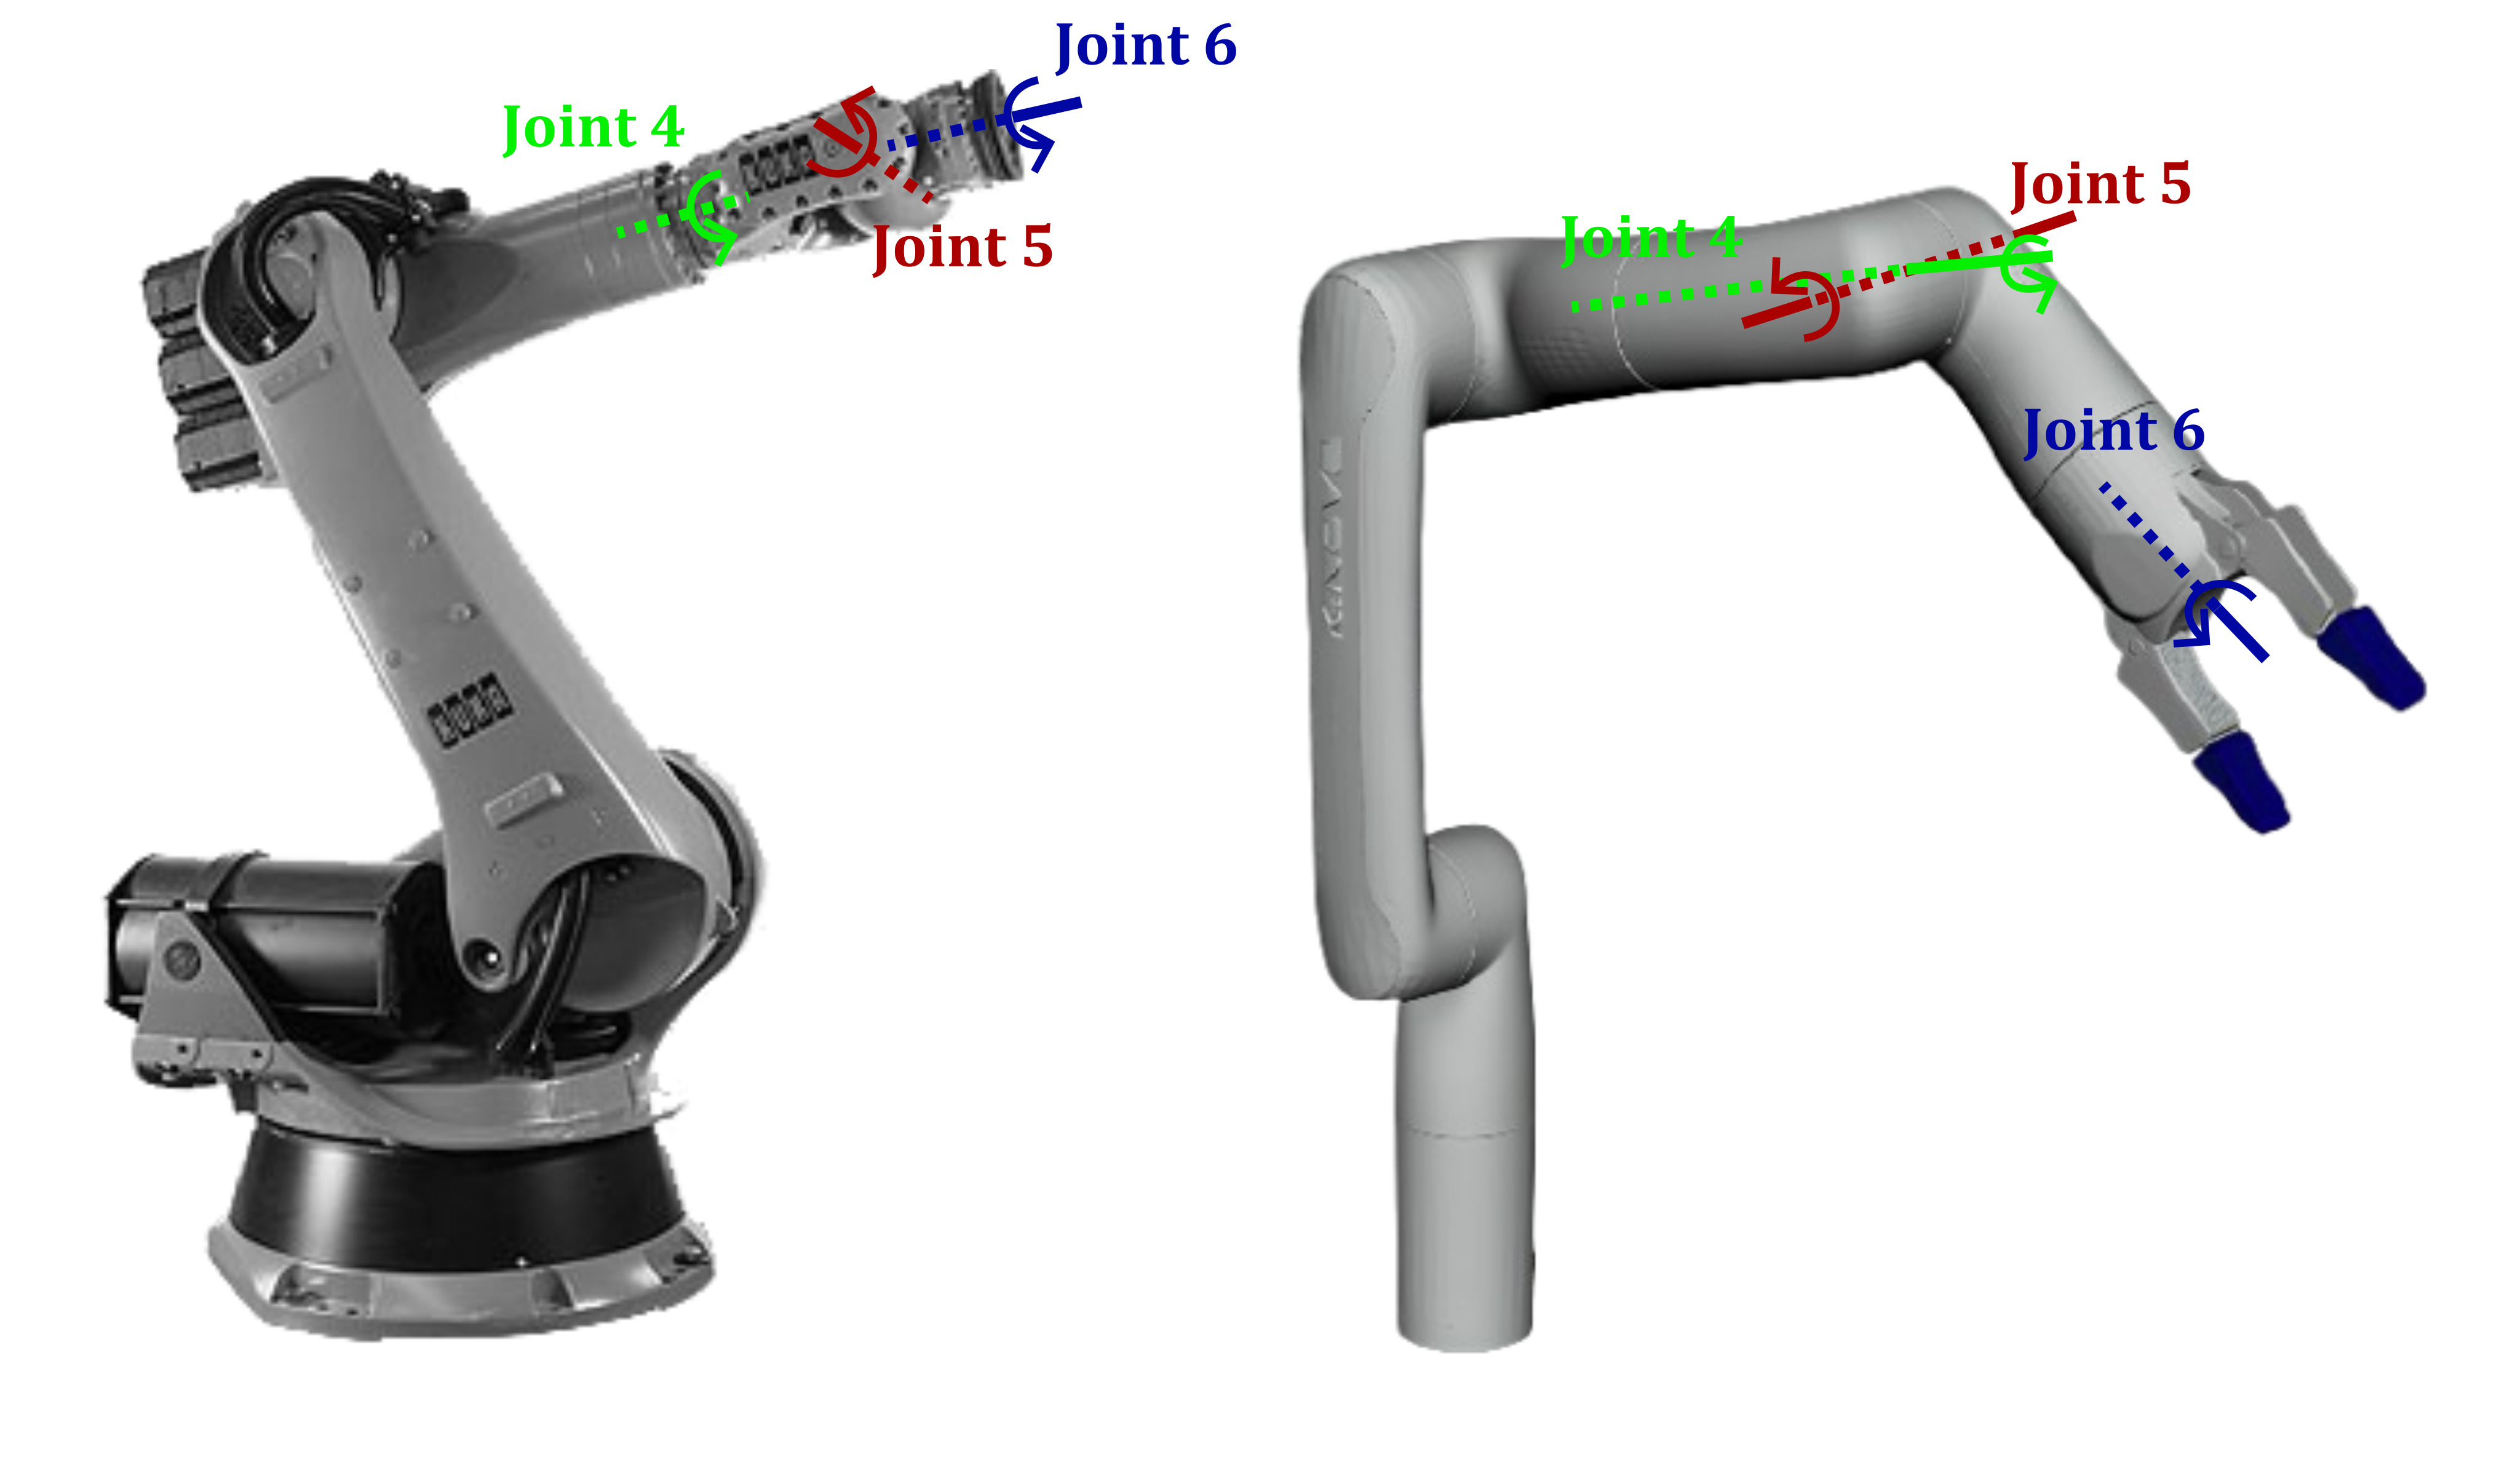
\includegraphics[width=0.90\textwidth]{Images/intro/p7_wrist_comparison.jpg}
\caption{(a) A KUKA KR-240 manipulator with a spherical wrist, whose final three axes intersect at a
common point and permit closed-form analytical inverse kinematics. (b) The Kinova Gen3 Lite, a
non-spherical wrist manipulator whose offsets between joints 4, 5 and 6 break kinematic
decoupling~\citep{sk2025diktracking}.}
\label{fig:intro_wrist}
\end{figure}

Modern industrial practice requires far more than standard pick-and-place operations. Tasks such as
continuous inspection and dynamic human-robot collaborative handoff increasingly require
manipulators to track end-effector trajectories whose target poses are determined online and cannot
be fully enumerated or precomputed in advance, in contrast to fixed, repeated motion profiles for
which offline trajectory planning remains both sufficient and
preferable~\citep{yoon2025reactive}. These operations require the manipulator to maintain a precise
end-effector pose along a continuous Cartesian path, which in turn requires joint velocity
resolution at the hardware's closed-loop control frequency. For non-spherical wrist manipulators
this introduces a fundamental kinematic bottleneck. The offset joint structure creates a unified,
non-linear system in which position and orientation are deeply coupled, requiring the inverse
kinematics to be solved as a single optimization at every control
timestep.

Classical solvers each fall short of this requirement in a different way. Iterative solvers such as
TRAC-IK~\citep{beeson2015trac} are widely used for their system-agnostic ability to handle joint
limits and multiple constraints, but even with a previous joint-state seed and a distance parameter
for solution selection, TRAC-IK remains fundamentally trajectory-unaware. Each waypoint is resolved
as an independent optimization with no inter-waypoint coupling, leading to configuration-branch
switching and joint-space discontinuities during continuous trajectory tracking. Heuristic methods
such as FABRIK~\citep{aristidou2011fabrik} are computationally efficient but limited to position
reaching and lack the necessary temporal awareness. Analytical closed-form solutions that reduce the
complex kinematics of the robot into a single 16th-degree polynomial to calculate all possible joint
configurations for a given pose~\citep{zohour2021kinova} cause the solver to jump between entirely
different joint configurations under continuous sub-millisecond tracking without strict nearest-joint
constraints.

Velocity-level controllers address this by operating directly in the differential domain.
Resolved-rate motion control~\citep{whitney1969resolved} computes joint velocities using the
Jacobian pseudo-inverse, damped least squares~\citep{wampler1986manipulator,chiaverini1994review}
introduces a damping factor to prevent velocity singularities, and quadratic velocity-level
programming formulations~\citep{zhang2013variable} further impose joint limit constraints explicitly,
offering safer hardware deployment. All of these methods, however, require an explicit, accurate
Jacobian at every timestep.

Despite these advances, trajectory tracking specifically on non-spherical wrist manipulators remains
unaddressed. The inverse kinematics solution introduces kinematic coupling that complicates both
analytical solvers and standard RL reward formulations, existing approaches either operate in torque
space requiring explicit dynamic models or augment pre-existing classical controllers rather than
learning from scratch, and no prior work demonstrates that a policy trained purely on static pose
reaching over a joint-limit-aware reachability dataset, without any trajectory supervision, can
generalize to continuous trajectory tracking at deployment~\citep{sk2025diktracking}.

The seventh study presents an end-to-end PPO-based differential inverse kinematics controller that
directly maps instantaneous Cartesian pose errors to joint velocity commands, bypassing any dependence on numerical solvers or explicit Jacobian
computation. A novel coupled reward function combining a min-operator pose reward, asymmetric
progress shaping, and an exponential joint velocity penalty enforces simultaneous position-orientation
convergence while producing smooth, hardware-safe velocity commands, and sim-to-real transfer is
validated on physical Kinova Gen3 Lite hardware at 20\,Hz. A compact $256\times256$ actor-critic
architecture, trained end-to-end on this coupled reward, learns a generalizable velocity-level
mapping. A controller trained purely on static, joint-limit-aware reachable-pose samples, with no
trajectory supervision, dynamic model, or task-specific retraining, generalizes zero-shot to four
continuous trajectory geometries, circle, square, lemniscate, and 3-D Lissajous, in both
simulation and on physical hardware, offering a reactive, online alternative to precomputed offline
IK pipelines for applications where target poses cannot be fully enumerated in
advance~\citep{sk2025diktracking}.

%% ------------------------------------------------------------
\subsection{Multi-Agent Learning for Cooperative Alignment}\label{subsec:intro_alpha}
%% ------------------------------------------------------------

Robot manipulation plays a key role in industrial automation tasks such as pick-and-place, sorting,
and assembly line inspection, which are increasingly handled by robotic systems. Robot movements are
based primarily on conventional methods such as kinematic and dynamic control, and on learning-based
approaches including imitation learning (IL) and reinforcement learning
(RL)~\citep{zare2024survey}. Conventional robotic control methods typically involve
modular pipelines consisting of sequential planning and control stages. These depend on accurate
kinematic or dynamic models, which are often complex and difficult to obtain in practice, and
predefined control sequences struggle to generalize across task variations without explicit
re-engineering of each module. Advancements in data-driven control techniques such as Learning from
Demonstration and data collection via teach pendants or teleoperation do not require explicit
knowledge of robot dynamics or environmental models to execute tasks. Although these approaches
eliminate the dependency on accurate dynamic models, they require a large volume of high-quality
data, so that the performance of such systems remains constrained by the availability and diversity
of the collected datasets, often making them difficult to scale in complex industrial
environments.

To overcome these limitations of data scarcity and human dependence on data collection,
reinforcement learning has been introduced as a powerful alternative~\citep{kober2013reinforcement}.
Unlike data-dependent IL and LfD, RL enables a robot to figure out optimal control policies through
interaction and exploration with the surroundings. Although RL methods require extensive training
time to converge, their capacity to learn optimal control robustly is often more reliable than
static data-driven approaches, and by optimizing a well-defined reward function RL-based agents can
potentially surpass the performance of human experts and develop resilient recovery behaviours that
are not represented in static datasets~\citep{gu2017deep}.

Although single-arm manipulation based on RL has demonstrated promising results in trajectory
optimization, intelligent pick-and-place, obstacle avoidance, and human-robot
interaction~\citep{yang2025gbagcrl}, complex tasks such as alignment and assembly of components
require collaborative manipulation rather than isolated single-arm execution. Extending RL from
single-agent to multi-agent systems poses significant challenges. In a single-agent environment, an
agent is concerned only with the outcomes of its own actions within a stationary distribution.
However, in multi-agent domains, an agent must account for both the consequences of its own actions
and the evolving behaviours of other agents. This interaction introduces non-stationarity into the
learning process, as the optimal policy of one agent becomes dependent on the fluctuating strategies
of its counterparts~\citep{nguyen2020deep}.

Multi-Agent Reinforcement Learning (MARL) was introduced to address these challenges by explicitly
modelling the interactions between multiple decision-making
entities~\citep{albrecht2024multi,low2025cooperative}. MARL methods are broadly classified along three primary axes, by cooperation structure, where
agents may be fully cooperative sharing a joint reward, fully competitive in zero-sum settings, or
mixed, by training and execution paradigm, spanning Independent Learning which treats other agents
as part of a non-stationary environment~\citep{dewitt2020independent}, Centralized Training with
Decentralized Execution (CTDE) which learns a shared critic while keeping independent policies at
execution, and Centralized Learning, and by communication protocol, separating agents that
explicitly share state or intent from those that must infer behaviour from observed actions. For
dual-arm manipulation, the problem is most effectively formulated as a fully
cooperative decentralized partially observable Markov Decision Process (Dec-POMDP) under the CTDE
paradigm~\citep{yu2022surprising}. While recent heterogeneous-agent CTDE methods such as
HAPPO offer monotonic improvement guarantees for asymmetric tasks via sequential policy
updates~\citep{kuba2021trust}, the agents in a symmetric dual-arm system are structurally symmetric,
each arm sharing identical architecture and observation dimensionality. In this homogeneous
cooperative setting, MAPPO's simultaneous update with a shared global-state critic is ideally
suited, directly capturing inter-arm spatial relationships during training while preserving
decentralized execution at deployment.

Despite the theoretical advantages of CTDE frameworks, their direct application to dual-arm
collaborative manipulation presents significant practical problems. Specifically, when agents are
required to simultaneously acquire low-level actuator skills and high-level inter-agent coordination
from scratch, sample efficiency degrades exponentially. Current dual-arm MARL approaches often rely
on rigid hand-designed action priors that do not adapt to different task phases. Furthermore, the
existing literature lacks a principled mechanism for smoothly transitioning between stable
single-arm priors and learned multi-agent coordination policies. This leaves the entire
computational burden on the MARL agents, ultimately limiting the scalability and sim-to-real
transferability of the learned controllers~\citep{alles2022learning}.

The eighth study proposes prior guided policy, a framework for dual-arm collaborative manipulation under the CTDE paradigm. A frozen single-arm PPO base policy provides stable
low-level actuator priors for reaching, while a MAPPO-based multi-agent coordination policy learns
inter-agent coordination and task-specific corrections through a learned adaptive gating scalar
$\alpha_{t}^{i}$, output as a seventh action dimension, that continuously interpolates between the
base prior and the coordination policy correction at every control timestep. Critically,
$\alpha_{t}^{i}$ is learned jointly with the coordination policy from timestep zero, allowing the
blending mechanism and coordination strategy to co-evolve. The two-phase task structure,
independent target reaching followed by cooperative alignment, is executed entirely under joint
velocity control, with gripper actuation and phase transitions handled by proximity thresholds. The
proposed framework is validated through direct sim-to-real transfer on physical Kinova Gen3 Lite
manipulators via the Kortex API, achieving 95.9\% reach and 93.9\% alignment success in simulation
(mean over three training seeds) and pick-and-pre-assembly alignment of square and cylindrical peg-in-hole configurations on hardware
at 20\,Hz, with a 200\,Hz policy inference rate on a CPU-only deployment
platform~\citep{sk2026priorguided}.

%% ============================================================
\section{Experimental Platform}\label{sec:intro_platform}
%% ============================================================

A common hardware platform runs through all eight studies, which is what allows the components
developed in one to be consumed directly by the next. The manipulator throughout is the Kinova Gen3
Lite, a 6-DOF serial arm whose non-spherical wrist is precisely what renders analytical inverse
kinematics intractable and motivates the learned controller of
Section~\ref{subsec:intro_dik}~\citep{sk2025diktracking}. Perception is provided by RGB-D sensing,
a global depth camera in simulation~\citep{sk2024bolthandling}, an Intel RealSense D415 fused with
the segmentation mask for size estimation~\citep{sk2024boltsorting}, wrist-mounted eye-in-hand
cameras for independent per-arm perception~\citep{sk2025sharedvision}, and YOLOv8 oriented bounding
box detection at 20--30 FPS for the planning and allocation
studies~\citep{surya2025iapf,sk2025competitive}. Integration spans Gazebo with ROS1 and ROS2 and the
ROS Kortex API for hardware communication, with control loops at 10--20\,Hz and a 200\,Hz policy
inference rate on a CPU-only platform~\citep{sk2025competitive,sk2026priorguided}. Validation progresses
from simulation only, to simulation and hardware, to direct sim-to-real transfer.
Table~\ref{tab:intro_results} collects the headline results.

% ---- TABLE: headline quantitative results ----
\begin{table}[htbp]
\centering
\caption{Headline quantitative results reported by the constituent studies.}
\label{tab:intro_results}
\resizebox{\textwidth}{!}{%
\begin{tabular}{cll}
\toprule
\textbf{Study} & \textbf{Metric} & \textbf{Result} \\
\midrule
1 & Bolt sorting in simulation                & No misclassifications on overlapping bolts \\
2 & Segmentation quality (DeepLabV3+)         & mIoU 0.95, best of PPLiteSeg~\citep{peng2022pp} / OCRNet~\citep{yuan2020object} / DeepLabV3+~\citep{chen2018encoder} \\
2 & Bolt sorting on real hardware             & No misclassifications and accurate size estimation \\ 
3 & Run-time role assignment                       & End-to-end in Gazebo/ROS2 and on physical hardware \\
4 & Inter-arm distance monitoring             & 16 link pairs tracked against a 0.1\,m safety threshold \\
5 & Vision detection accuracy (YOLOv8 OBB~\citep{yolov8})    & 0.99 bolts / 0.97 nuts at 20 FPS \\
6 & Velocity improvement over fixed allocation & $\approx$47\% (homogeneous), zero collisions \\
6 & Mixed-object overhead                     & $\approx$11\%, offset by superior safety margins \\
7 & Zero-shot trajectory generalization       & Circle, square, lemniscate, 3-D Lissajous at 20\,Hz \\
8 & Reach / alignment success (simulation, 3-seed mean) & 95.9\% reach, 93.9\% alignment \\
8 & Reach / alignment success (hardware)    & 93.3\% reach, 90.0\% alignment \\
\bottomrule
\end{tabular}%
}
\end{table}

%% ============================================================
\section{Research Gaps}\label{sec:intro_gaps}
%% ============================================================

Taken together, the discussion above identifies the following gaps, each addressed by one of the
studies in this thesis.

\begin{description}
    \item[G1. Perception for small, low-feature components.] Existing research on object sorting
    faces limitations in handling densely packed objects with limited visual features, and existing
    methods suffer from limitations in accuracy, speed, and adaptability while often requiring
    multiple sensors that increase system complexity and cost~\citep{sk2024bolthandling}. Classical
    localization is unreliable under varying light conditions, shapes, and
    colours~\citep{sk2024boltsorting}.

    \item[G2. Runtime arm selection from onboard perception.] Coordination has been addressed by
    control-level coupling, by centrally solved scheduling from an external view, or by offline
    static workspace zoning. A second arm's own eye-in-hand camera has not been used to decide which
    arm should manipulate a shared target at runtime~\citep{sk2025sharedvision}.

    \item[G3. Sensor-free, real-time inter-arm distance.] Conventional collision detection either
    depends on external sensors or on computationally expensive algorithms that compromise real-time
    applicability, and classical geometric formulations provide only discrete detection without the
    continuous distance metrics that modern controllers require for smooth motion
    planning~\citep{sk2025distance,surya2025iapf}.

    \item[G4. Stable asymmetric dual-arm motion planning.] Asymmetric coordinated manipulation
    enables a wider range of complex tasks but is more challenging, and APF methods face unique
    difficulties related to workspace sharing and coordinated manipulation in manufacturing
    contexts~\citep{surya2025iapf,sk2025competitive}.

    \item[G5. Competitive task allocation.] Current industrial practice assigns fixed object types
    to each arm and fails when objects appear outside designated zones. Existing systems rely on
    predetermined trajectories and rigid allocation strategies, causing suboptimal workspace
    utilization and collision risks~\citep{sk2025competitive}.

    \item[G6. Trajectory tracking on non-spherical wrists.] The violation of kinematic decoupling
    renders analytical IK intractable, and classical velocity-level controllers require an explicit,
    accurate Jacobian at every timestep. The work demonstrates that a policy trained, without trajectory supervision, generalizes to continuous trajectory
    tracking at deployment~\citep{sk2025diktracking}.

    \item[G7. Sample-efficient dual-arm coordination learning.] When agents must simultaneously
    acquire low-level actuator skills and high-level coordination from scratch, sample efficiency
    degrades exponentially, and the literature lacks a principled mechanism for smoothly
    transitioning between stable single-arm priors and learned multi-agent coordination
    policies~\citep{sk2026priorguided}.
\end{description}

% ---- TABLE: summary of the constituent studies ----
\begin{table}[htbp]
\centering
\caption{Summary of the studies constituting this thesis, in the order they are developed.}
\label{tab:intro_studies}
\resizebox{\textwidth}{!}{%
\begin{tabular}{clllc}
\toprule
\textbf{\#} & \textbf{Theme} & \textbf{Core method} & \textbf{Platform / validation} & \textbf{Gap} \\
\midrule
1 & Perception        & $k$-means + Oriented Chamfer matching on RGB-D & Gazebo (ROS1), Kinova Gen3 Lite & G1 \\
2 & Perception        & DeepLabV3+~\citep{chen2018encoder} segmentation + classical vision, depth fusion & Hardware, RealSense D415 & G1 \\
3 & Dual-arm coordination & Eye-in-hand ArUco~\citep{garrido2014automatic} search, reachability role assignment & Gazebo/ROS2 + dual-arm hardware & G2 \\
4 & Safety            & Line-segment kinematic inter-arm distance matrix & Dual Kinova Gen3 Lite hardware & G3 \\
5 & Motion planning   & iAPF with PD angular control, empirical validation & Hardware, YOLOv8 OBB~\citep{yolov8} at 20 FPS & G4 \\
6 & Task allocation   & Competitive allocation, temporal proposal windows & Dual-arm hardware & G5 \\
7 & Learned control   & PPO~\citep{schulman2017proximal} differential IK, coupled reward & Sim-to-real, Kinova Gen3 Lite at 20\,Hz & G6 \\
8 & Learned control   & MAPPO~\citep{yu2022surprising} with adaptive gating over a frozen PPO prior & Sim-to-real, CPU-only deployment at 20 Hz & G7 \\
\bottomrule
\end{tabular}%
}
\end{table}

%% ============================================================
\section{Research Contributions}\label{sec:intro_contributions}
%% ============================================================

The contributions of this thesis, in the order the studies are developed, are as follows.

\begin{description}
    \item[C1. Vision-based bolt handling with RGB-D template matching.] $k$-means segmentation
    with Oriented Chamfer matching on RGB-D point clouds for pose estimation, with colour-based
    segmentation, template matching and contour analysis for size estimation, achieving bolt sorting without misclassifications on overlapping bolts in Gazebo~\citep{sk2024bolthandling}.

    \item[C2. Deep-learning segmentation fused with classical vision.] A custom bolt dataset
    spanning environmental conditions and both new and aged bolts, a comparative analysis in which
    DeepLabV3+ reached an mIoU of 0.95 over PPLiteSeg and OCRNet, and fusion of the segmentation
    mask with RealSense D415 depth to localize and sort bolts by size~\citep{sk2024boltsorting}.

    \item[C3. Runtime reachability-based role assignment.] A per-detection rule selecting the
    acting arm by minimum base-to-target distance, and a cross-frame pose relay expressing a target
    seen by one arm's eye-in-hand camera in the other arm's base frame, so reachability is evaluated
    for both arms without a shared external sensor. Validated end-to-end in Gazebo/ROS2 and on
    hardware~\citep{sk2025sharedvision}.

    \item[C4. Kinematics-based inter-arm distance monitoring.] A geometric framework classifying
    link configurations as parallel, intersecting, or skew, specialized from $n$ arms to the
    dual-arm table-mounted case, constructing distance matrices from joint feedback alone with no
    external sensors~\citep{sk2025distance}.

    \item[C5. iAPF for asymmetric dual-arm motion planning.] A three-way force equilibrium with
    velocity-dependent stabilization, coupling iAPF linear velocity control to PD-regulated angular
    velocity, empirically validated for smooth, stable convergence, driven by YOLOv8 OBB detection
    at 20 FPS with 0.99/0.97 accuracy for bolts/nuts~\citep{surya2025iapf}.

    \item[C6. Competitive task allocation with temporal proposal windows.] Distance-based
    allocation in which each arm evaluates detections over five consecutive frames before
    committing, with spatial conflict resolution at 0.01\,m, giving $\approx$47\% average velocity
    improvement over fixed allocation with zero collisions~\citep{sk2025competitive}.

    \item[C7. Coupled-reward differential inverse kinematics.] A reward architecture combining
    min-operator pose coupling, asymmetric progress shaping, and an exponential joint velocity penalty that
    resolves simultaneous position-orientation convergence without staged curricula, generalizing
    zero-shot from static pose reaching to four continuous trajectory
    geometries~\citep{sk2025diktracking}.

    \item[C8. Prior guided policy learning.] A learned gating scalar, emitted as a
    seventh action dimension, that interpolates between a frozen single-arm PPO prior and a MAPPO
    coordination correction at every timestep and co-evolves with the coordination policy from
    timestep zero. 95.9\% reach and 93.9\% alignment success in simulation (three-seed mean) with sim-to-real transfer
    on a CPU-only platform~\citep{sk2026priorguided}.
\end{description}

%% ============================================================
\section{Thesis Organization}\label{sec:intro_organization}
%% ============================================================

The remainder of this thesis is structured as follows.

\begin{description}
    \item[Chapter 2] reviews the literature underpinning the four themes of this work, template
    matching and segmentation for low-textured objects, size estimation from RGB-D information,
    dual-arm coordination, motion planning and task allocation, collision detection and artificial potential field methods, and learning-based approaches to inverse kinematics and multi-agent manipulation.

    \item[Chapter 3] presents the vision pipelines for automated bolt handling and sorting, covering
    RGB-D point-cloud segmentation with Oriented Chamfer matching, deep-learning-based semantic
    segmentation, depth-based size estimation, and localization in the robot's configuration.

    \item[Chapter 4] develops the dual-arm shared-vision system, covering independent eye-in-hand
    search, cross-frame pose relay through a fixed inter-arm transform, the reachability-based
    role-assignment rule, and damped least-squares resolved-rate control.

    \item[Chapter 5] derives the kinematics-based inter-arm distance framework, covering the
    classification of link configurations as parallel, intersecting, or skew, the general $n$-arm
    formulation, its dual-arm specialization, and distance-matrix construction for collision
    monitoring, purely as a mathematical and sensing contribution, independent of any motion-planning or trajectory content.

    \item[Chapter 6] introduces the iAPF motion planning framework built on the distance signal of
    Chapter 5, covering the three-way force equilibrium, vision-based pose estimation, the hybrid
    linear-angular controller, and the priority-lock coordination mechanism, together with its
    experimental validation under a fixed object-to-arm
    assignment.

    \item[Chapter 7] presents the distance-based competitive task allocation mechanism that replaces
    Chapter 6's fixed object-to-arm assignment with a runtime, temporal-window decision, reusing the
    iAPF controller unchanged as its execution layer, together with its simulation and hardware
    validation.

    \item[Chapter 8] presents the learning-based controllers, covering the coupled-reward
    differential inverse kinematics formulation for non-spherical wrist trajectory tracking and the
    prior guded policy learning architecture for cooperative dual-arm pre-assembly alignment,
    together with their sim-to-real validation.

    \item[Chapter 9] concludes with a summary of contributions, a discussion of limitations, and
    directions for future work.
\end{description}
